\documentclass[12pt]{article}
\usepackage[english]{babel}
\usepackage[utf8]{inputenc}
\usepackage{amsmath, amssymb, amsthm}
\usepackage{graphicx}
\usepackage{hyperref}
\usepackage[margin=.75in]{geometry}
\usepackage{xcolor}
\usepackage{algorithm}
\usepackage[noend]{algpseudocode}
\usepackage{hyperref}
\hypersetup{
    colorlinks=true,
    urlcolor=blue,
    linkcolor=black,
    }

\newcommand{\id}{\text{id}}
\newcommand{\od}{\text{od}}

\setlength{\topmargin}{0pt}
\setlength{\headsep}{0pt}
\textheight = 600pt

\newtheorem{theorem}{Theorem}
\newtheorem{corollary}{Corollary}
\newtheorem{lemma}{Lemma}
\newtheorem{rrule}{Reduction Rule}
\newtheorem{prule}{Pruning Rule}

\title{Pruning Rules for Edge Clique Cover}
\author{Ben Kallus}
\date{}

\begin{document}
\maketitle

\section*{Abstract}

    Covering the edges of a graph with the minimum number of complete subgraphs is an NP-hard problem.
    We expand upon a previous branch-and-reduce method for this solving problem by Gramm et al. with improvements to previously-known data reduction rules, as well as new pruning rules that significantly reduce the portion of the search tree to be explored.

\section*{Introduction}

    The problem of covering the edges of a graph with complete subgraphs, called the edge clique cover problem, has been of interest to graph theorists since at least the 1960s. %% www.renyi.hu/~p_erdos/1966-21.pdf
    More recently, applications of the problem have surfaced in compiler optimization, computational geometry, and applied statistics. %% This is basically stolen from Gramm, but can't find other good applications.
    The edge clique cover problem is NP-hard, indicating that it is unlikely that a polynomial-time algorithm for the problem will be found.
    The problem is also APX-hard, so an approximation algorithm accurate to within a constant factor of $2^k$ does not exist for any $k < 2$ unless P = NP. %% citation needed
    Thus, polynomial-time heuristic algorithms, such as the one introduced by Conte et al., can offer only no meaningful guarantees about accuracy. %% Citation needed
    Gramm et al. introduced data reductions that provide a significant improvement over brute-force computation when solving the problem exactly in practice for sparse graphs, and are believed to be asymptotically optimal. %% https://epubs.siam.org/doi/pdf/10.1137/1.9781611973105.75
    However, their algorithm can have prohibitive running time on dense graphs, due in part to its exhaustively exploring and reexploring the search tree through iterative deepening.
    We expand upon the work by Gramm et al. with new pruning rules that, when employed within a branch-and-bound framework, allow for computing minimum edge clique covers with significantly improved running time.

\section*{Preliminaries}

\subsection*{Definitions}
    A \textbf{graph} $G$ is a collection of vertices $V(G)$ together with a collection of edges $E(G) \subseteq \{uv \mid u,v \in V(G)\}$.
    We consider only simple, undirected, unweighted graphs.
    Thus, each edge $e \in E(G)$ is a 2-element unordered subcollection of $V(G)$.
    Self-loops are not permitted, and any pair of distinct vertices in $V(G)$ is joined by at most one edge.
    The \textbf{neighborhood} of a vertex $v$, denoted $N(v)$, is the set of vertices $\{u \mid uv \in E(G)\}$.
    The \textbf{closed neighborhood} of a vertex $v$, denoted $N[v]$, is $N(v) \cup \{v\}$.
    The \textbf{complete graph} of order $n$, denoted $K_n$, is the unique (up to isomorphism) graph on $n$ vertices in which $uv \in E(K_n)$ for all distinct $u,v \in V(K_n)$.
    A \textbf{subgraph} of a graph $G$ is a graph $H$ such that $V(H) \subseteq V(G)$ and $E(H) \subseteq E(G)$.
    The subgraph of $G$ \textbf{induced} by a vertex set $C \subseteq V(G)$, denoted $G[C]$, is the subgraph of $G$ with $V(G[C]) = C$ and $E(G[C]) = \{uv \in E(G) \mid u, v \in C\}$.
    A \textbf{$k$-clique} in an undirected graph $G$ is a set $C \subseteq V(G)$ of order $k$ such that $G[C]$ is complete.
    For example, in the graph shown in Figure 1, $\{a, b, c\}$ is a 3-clique.
    \begin{figure}[hbt!]
    \begin{center}
        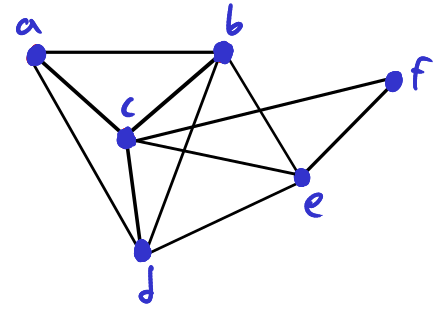
\includegraphics[scale=.6]{fig1.png} % highlight a, b, c
        \caption{}
    \end{center}
    \end{figure}

    Note that a clique may be a proper subset of another clique.
    For example, in Figure 1, the 3-clique $\{a, b, c\}$ is proper subset of the 4-clique $\{a, b, c, d\}$.
    The 4-clique $\{a, b, c, d\}$ is not a proper subset of any other clique in the graph, so we say $\{a, b, c, d\}$ is a \textbf{maximal clique}.
   
\subsection*{The Edge Clique Cover Problem}

    An edge clique cover for an undirected graph $G$ is a collection $\mathcal C$ of cliques in $G$ such that for all $uv \in E(G)$, $u, v \in C$ for some $C \in \mathcal C$.\footnote{Note that isolated vertices have no effect on an edge clique cover, because they are incident to no edges. Thus, we consider only graphs without isolated vertices.}
    For example, $\mathcal C_1 = \{\{a, b, c, d\}, \{c, e, f\}, \{d, e\}, \{b, e\}\}$ constitutes an edge clique cover for the graph from Figure 1.
    \begin{figure}[hbt!]
    \begin{center}
        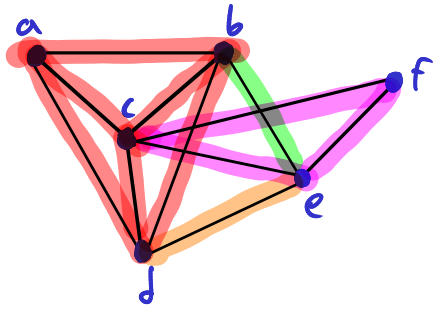
\includegraphics[scale=.6]{fig2.png}

        \caption{The edge clique cover $\mathcal C_1$}
    \end{center}
    \end{figure}
    
    Observe that $\mathcal C_1$ is not of minimum cardinality; the 2-cliques $\{d,e\}$ and $\{b,e\}$ can be substituted for the 3-clique $\{b, d, e\}$ to construct a new edge clique cover $\mathcal C_2$ of cardinality 3.
    \begin{figure}[hbt!]
    \begin{center}
        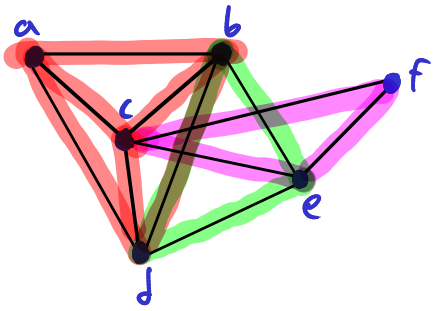
\includegraphics[scale=.6]{fig3.png}

        \caption{The edge clique cover $\mathcal C_2$}
    \end{center}
    \end{figure}
    The graph from Figure 1 cannot be covered by any fewer than 3 cliques, so $\mathcal C_2$ is an edge clique cover of minimum cardinality.
    Note that a graph may have many minimum edge clique covers; $\mathcal C_3 = \{\{a, b, c, d\}, \{c, e, f\}, \{b, c, d, e\}\}$ is another minimum edge clique cover for the graph from Figure 1.
    The \textbf{edge clique cover number} of a graph $G$, $\text{ecc}(G)$, is the cardinality of a minimum edge clique cover for $G$.

\section*{Related Work}

    The edge clique cover problem was first introduced as the intersection number problem in 1966. %% file:///tmp/mozilla_bkallus0/1966-21.pdf
    In 1973, Kellerman produced the first heuristic algorithm for the edge clique cover problem %% Kellerman, E. Determination of keyword conflict. IBM Tech. Disclosure Bull. 16, 2 (July 1973), 544-546.
    This was improved by Kou et al. in 1978.
    Additionally, Kou et al. showed through a reduction to and from the related vertex clique cover problem that the edge clique cover problem is NP-complete.
    The vertex clique cover problem, one of Richard Karp's original 21 NP-complete problems, is the problem of finding a minimum cardinality set of cliques in a graph such that every vertex in the graph is included in at least one clique.
    An arguably more famous formulation of the vertex clique cover problem is the graph coloring problem, which asks for the fewest number of colors in a coloring of the graph's vertices such that no two adjacent vertices share a color.
    It is clear to see that the graph coloring problem is equivalent to the vertex clique cover problem on the complement graph.
    
    Existing techniques for edge clique cover involve 

\newpage\subsection*{Existing Reduction Rules}

    Gramm et al. introduce four polynomial-time reduction rules for the edge clique cover problem.
    Each of these provides a condition under which either the problem instance can be reduced in size or difficulty, or a portion of the solution can be deduced.
    They can be applied in any order.
    We restate them here without proof.

    \begin{rrule}
        Remove isolated vertices and vertices incident only to covered edges.
    \end{rrule}

    \begin{rrule}
        If an uncovered edge participates in exactly one maximal clique $C$, cover $C$.
    \end{rrule}

    \begin{rrule}
        Suppose that there exists a vertex $v$ such that $N[u] \subseteq N[v]$ for some vertex $u \in N(v)$.
        Then, we call $u$ a prisoner of $v$.
        An exit of $v$ is a vertex in $N(v)$ that is not a prisoner of $v$.
        If every prisoner of $v$ is adjacent to at least one vertex other than $v$ via an uncovered edge, and every exit of $v$ is adjacent to at least one prisoner of $v$, remove $v$ and insert it into any clique containing a prisoner of $v$ covered from now on.
    \end{rrule}

    \begin{rrule}
        For each vertex $v$ such that the subgraph $H$ induced by $N(v)$ is disconnected, delete $v$ and replace it with one new vertex for each component of $H$.
        Connect each new vertex to each vertex in its corresponding component with a new edge, maintaining the covered status of the corresponding edge from $v$.
        Once a cover has been computed, replace all instances of the new vertices created by this reduction rule in the clique cover with $v$.
    \end{rrule}


\section*{Contributions}

\subsection*{Correction to Reduction Rule 3}

    \begin{figure}[hbt!]\begin{center}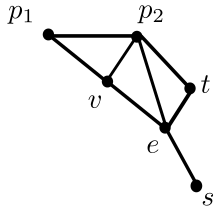
\includegraphics[scale=.6]{g.png}\end{center} \caption{The graph $G$, with labeled vertices.} \label{fig:rulethreebad}\end{figure}
    As stated above and by Gramm et al., Reduction Rule 3 is incorrect.
    The following series of reductions will compute an invalid edge clique cover for the graph $G$ in \ref{fig:rulethreebad} by exploiting an interaction between Reduction Rule 1 and Reduction Rule 3.
    \begin{enumerate}
        \item Apply Rule 2 to the edge $et$ to cover the clique $\{e, t, p_2\}$.
        \item Apply Rule 1 to the vertex $t$ to remove it from the graph.
        \item Apply Rule 3 to the vertex $v$ to remove it from the graph. Note that its prisoners are $p_1, p_2$, and its only exit is $e$.
        \item Apply Rule 2 to the edge $p_1p_2$ to cover the clique $\{p_1, p_2, v\}$. Note that $v$ is added to this clique because of Reduction Rule 3.
        \item Apply Rule 2 to the edge $es$ to cover the clique $\{e, s\}$.
    \end{enumerate}
    
    \begin{figure}[hbt!]
        \begin{center}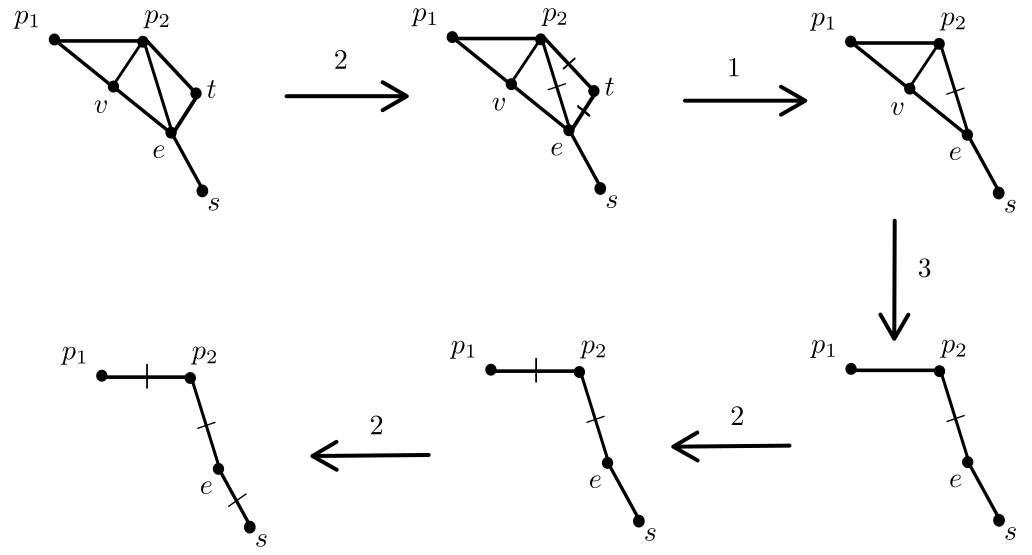
\includegraphics[width=\linewidth]{rule_three_failure.png}\end{center}
            \caption{The series of reductions applied to $G$.}
    \end{figure}

    Following this series of reductions, all edges in the reduced graph are covered, so we are to assume that $\{\{e, t, p_2\}, \{p_1, p_2, v\}, \{e, s\}\}$ is a minimum edge clique cover for $G$.
    However, this set does not cover the edge $ve$, and so it is not an edge clique cover at all.
    To account for this counterexample, we propose a modification to Reduction Rule 3.
    
   \medskip\noindent\textbf{Modified Reduction Rule 3.} {\it Suppose that there exists a vertex $v$ such that $N[u] \subseteq N[v]$ for some vertex $u \in N(v)$.
        Then, we call $u$ a prisoner of $v$.
        An exit of $v$ is a vertex in $N(v)$ that is not a prisoner of $v$.
        If every prisoner of $v$ is adjacent to at least one vertex other than $v$ via an uncovered edge, and every exit of $v$ is adjacent to at least one prisoner of $v$ {\bf via an uncovered edge}, remove $v$ and insert it into any clique containing a prisoner of $v$ covered from now on.}
    \medskip

    In the proof of Reduction Rule 3's correctness by Gramm et al., they assert that an edge $\{v, e\}$ from a vertex $v$ to one of its exits $e$ must be in a clique with at least one of the prisoners adjacent to $e$.
    However, that assertion does not necessarily hold if $pe$ is covered for every prisoner $p$ adjacent to $e$.
    Clearly, Modified Reduction Rule 3 avoids this issue by ensuring that $e$ is adjacent to at least one prisoner via an uncovered edge.

\subsection*{Pruning Rules}

    In the search tree algorithm by Gramm et al. computes edge clique covers incrementally through recursive branching and reduction.
    We provide pseudocode for their algorithm below. %% CITE
    \begin{algorithm}
    \caption{Branch-and-reduce algorithm from Gramm et al.}    
    \begin{algorithmic}
        \State \textbf{Input}: A graph $G$.
        \State \textbf{Output}: A minimum edge clique cover for $G$.
        \State $k \gets 0$
        \State $X \gets \textbf{nil}$
        \While{X = \textbf{nil}}
            \State $X \gets \Call{branch}{G, k, \emptyset}$
            \State $k \gets k + 1$
        \EndWhile
        \State \textbf{return} $X$
        \Function{branch}{$G, k, X$}
            \If{$X$ covers $G$}
            \State \textbf{return} $X$
            \EndIf
            \State \Call{reduce}{$G, k, X$}
            \If{$k < 0$}
                \State \textbf{return nil}
            \EndIf
            \State $e \gets$ an edge of minimum score in $G$
            \For{\textbf{each} maximal clique $C$ in $G$ containing $e$}
                \State $X' \gets$ \Call{branch}{$G, k-1, X \cup \{C\}$}
                \If{$X' \neq \textbf{nil}$}
                    \State \textbf{return} $X'$
                \EndIf
            \EndFor
            \State \textbf{return nil}
        \EndFunction
    \end{algorithmic}
    \end{algorithm}
    
    Because of this algorithm's iterative deepening approach, the first edge clique cover found is always of minimum cardinality.
    However, large amounts of computational time are spent computing and recomputing partial covers.
    It is for this reason that we do away with the iterative deepening in our reimplementation of Gramm et al.'s work.
    A simple optimization to eliminate wasted search time is to track the size $s$ of the smallest edge clique cover found so far.
    If at any point the search tree algorithm adds $s$ cliques during the construction of a cover, that branch of the search cannot lead to a minimum edge clique cover, and can therefore be ignored.
    This simple pruning can be augmented through the use of a lower bound $\ell$ on the number of cliques remaining to cover.
    If at any point the search tree algorithm adds $s  - \ell$ cliques during the construction of a cover, that branch of the search can be ignored as well.
    Thus, in this branch-and-bound model, if a large lower bound can be obtained quickly, large portions of the search tree can be ignored.
    We provide pseudocode for this algorithm below.
    \begin{algorithm}
    \caption{Branch-and-bound algorithm}    
    \begin{algorithmic}
        \State \textbf{Input}: A graph $G$.
        \State \textbf{Output}: A minimum edge clique cover for $G$.
        \State $k \gets \frac{|V(G)|^2}{2}$ \Comment{This is a well-known upper bound on $\text{ecc}(G)$}
        \State $X \gets \Call{branch}{G, k, \emptyset}$
        \State \textbf{return} $X$
        \Function{branch}{$G, k, X$}
            \State \Call{reduce}{$G, k, X$}
            \If{$|X| \geq k$}
                \State \textbf{return nil}
            \Else\If{$X$ covers $G$}
                \State \textbf{return} $X$
            \EndIf
            \EndIf
            \State $e \gets$ an edge of minimum score in $G$
            \State $\ell \gets$ \Call{compute-lower-bound}{$G, k, X$}
            \If{$|X| + \ell \geq k$}
                \State \textbf{return nil}
            \EndIf
            \State $B \gets X$
            \For{\textbf{each} maximal clique $C$ in $G$ containing $e$}
                \State $X' \gets$ \Call{branch}{$G, k, X \cup \{C\}$}
                \If{$X' \neq \textbf{nil}$}
                    \State $k \gets |X'|$
                    \State $B \gets X'$
                \EndIf
            \EndFor
            \State \textbf{return} $B$
        \EndFunction
    \end{algorithmic}
    \end{algorithm}

    We now provide two techniques for computing a lower bound suitable for pruning.
    It is well known that for a graph $G$ with no isolated vertices, the size of a maximum vertex independent set in $G$ is a lower bound for $\text{ecc}(G)$.
    We propose a pruning rule based on this bound.
    \begin{algorithm}
    \caption{Vertex set lower bound}
    \begin{algorithmic}
        \State \textbf{Input} A graph $G$, a set $X$ of covered cliques in $G$.
        \State \textbf{Output} A lower bound for the number of cliques necessary to add to $X$ to produce an edge clique cover.
        \State $I \gets \emptyset$.
        \For{\textbf{each} vertex $v \in V(G)$}
            \If{$v$ is adjacent to an edge not in a clique in $X$ \textbf{and} $I \cup \{v\}$ is an independent set}
                \State $I \gets I \cup \{v\}$
            \EndIf
        \EndFor
        \State \textbf{return} $|I|$
    \end{algorithmic}
    \end{algorithm}

    We now prove this lower bound's correctness.
    \begin{proof}
        Because $I$ is an independent set, no two vertices in $I$ can be in the same clique in $G$.
        Because each vertex in $I$ is incident to an uncovered edge, each vertex in $I$ must be contained in at least one clique yet to be added to $X$.
        Thus, at least $|I|$ cliques must be added to $X$ to produce an edge clique cover.
    \end{proof}

    We improve upon this lower bound with a second.
    Another well-known lower bound for $\text{ecc}(G)$ is the size of a maximum independent set of edges in $G$.
    We propose a second pruning rule based loosely on this bound.
    \begin{algorithm}
    \caption{Edge set lower bound}
    \begin{algorithmic}
        \State \textbf{Input} A graph $G$, a set $X$ of covered cliques in $G$.
        \State \textbf{Output} A lower bound for the number of cliques necessary to add to $X$ to produce an edge clique cover.
        \State $I \gets \emptyset$.
        \For{\textbf{each} edge $uv \in E(G)$ that is not covered by a clique in $X$}
            \State $valid \gets \textbf{true}$
            \For{\textbf{each} edge $xy \in I$}
                \If{$uv$ and $xy$ do not share a vertex \textbf{and} $\{u, v\} \cup \{x, y\}$ induces a $K_4$ in $G$}
                    \State $valid \gets \textbf{false}$
                    \State \textbf{break}
                \EndIf
                \If{$uv$ and $xy$ share a vertex \textbf{and} $\{u, v\} \cup \{x, y\}$ induces a $K_3$ in $G$}
                    \State $valid \gets \textbf{false}$
                    \State \textbf{break}
                \EndIf
            \EndFor
            \If{$valid$}
                \State $I \gets I \cup \{uv\}$
            \EndIf
        \EndFor
        \State \textbf{return} $|I|$
    \end{algorithmic}
    \end{algorithm}

    \begin{figure}[hbt!]
        \begin{center}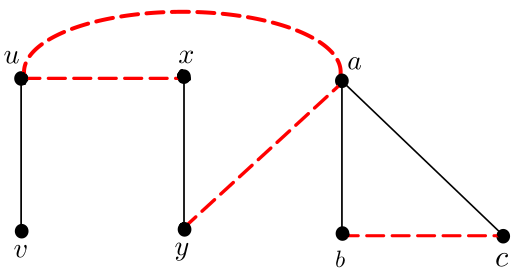
\includegraphics[scale=.7]{7.png}\end{center}
            \caption{}
        \label{fig:edgerule}
    \end{figure}
    
    Figure \ref{fig:edgerule} demonstrates the intuition behind the edge pruning rule.
    For each pair of black edges in Figure \ref{fig:edgerule}, there is at least one edge missing between them, emphasized in red.
    Thus, no two of $uv, xy, ab, ac$ can belong to a clique together, so at least four cliques remain to be covered.
    We now prove this lower bound's correctness.
    \begin{proof}
        Let $uv, xy \in I$.
        Suppose that $uv, xy$ do not share a vertex.
        Then, the construction of $I$ ensures that $\{u, v\} \cup \{x, y\}$ does not induce a $K_4$ in $G$.
        Thus, at least one of $ux, uy, vx, vy$ is not an edge in $G$, so $uv$ and $xy$ cannot participate in a clique together in $G$.
        Now, suppose without loss of generality that $u = x$.
        Then, the construction of $I$ ensures that $\{u, v\} \cup \{x, y\} = \{u, v, y\}$ does not induce a $K_3$ in $G$.
        Thus, $vy$ is not an edge in $G$, so $uv$ and $xy = uy$ cannot participate in a clique together in $G$.
        Thus, no two edges in $I$ belong to a clique together in $G$.
        Thus, because each edge in $I$ is uncovered, at least $|I|$ cliques must be added to $X$ to produce an edge clique cover.
    \end{proof}

\section*{Implementation}

    We implemented both the branch-and-reduce algorithm by Gramm et al. and our contributions to it in 762 lines of C++ code, excluding comments and whitespace.
    Our program and source code are available \href{https://github.com/kenballus/ecc-reductions}{here}.
    We represent graphs using simple adjacency lists, implmented using \texttt{vector} from the g++ STL.

\section*{Experiments}

\subsection*{Experimental Setup}

    Experiments were run on an AMD Ryzen 5 3600 with 16 GB of system memory running Arch Linux with a 5.12.4 kernel.
    The program was written in C++20, and compiled using g++ 11.1.0 with the \texttt{-O3} and \texttt{-march=native} optimization flags.

\section*{Future Directions}

    Because the search tree algorithm by Gramm et al. requires the enumeration of all maximal cliques containing the branching edge, it breaks dow when the branching edge participates in a number of maximal cliques that cannot be easily enumerated.
    It remains to be seen whether a better branching heuristic can minimize the total degree of the search tree to a greater extent than selecting the lowest score edge.
    Reduction Rule 4, as described by Gramm et al., does not improve the running time of the search tree algorithm because the cost of introducing new vertices outweights the benefit of removing a potentially high-degree vertex.
    It is possible that selective application of Reduction Rule 4, such as applying it only to cut-vertices, could minimize the negative impact of the rule by guaranteeing that new components are created in the graph.

\end{document}
